%%%--- Template for master thesis at SfS
%%%--- Modified template with more comments and examples -- SG, 11/06/09
%%%------
\documentclass[11pt,a4paper,twoside,openright]{report}
%%not needed \usepackage{E}
\usepackage[english]{ETHDAsfs}%--> ETHDASA + fancyheadings + ... "umlaute"
%  + sfs-hyper -> hyperref

\usepackage{pdfpages}%%to include the confirmation of originality (plagiarism
\usepackage{amsbsy}%% for \boldsymbol and \pmb{.}
\usepackage{amssymb}%% calls  amsfonts...
%or \usepackage{german8}%-- =  german  +  isolatin1
\usepackage{graphicx}%-- f�r PostScript-Grafiken (besser als  psfig!)
%\usepackage[draft]{graphicx} % grafics shown as boxes --> faster compilation
% \addbibresource{biblio.bib}

\usepackage[longnamesfirst]{natbib}%was {sfsbib}%- F�r  Literatur-Referenzen
%           ^^^^^^^^^^^^^^ 1) "Hampel, Ronchetti, ..,"  2) "Hampel et al"
% Engineers (and other funny people) want to see [1], [2]
% ---> use 'numbers' : \usepackage[longnamesfirst,number]{natbib}
%
%
\usepackage{texab}%- 'tex Abk�rzungen' /u/sfs/tex/tex/latex/texab.sty
        %%- z.B.  \R, \Z, \Q, \Nat f�r reelle, ganze, rationale, nat�rl. Zahlen;
        %%-       \N   (Normalvert.)  \W == Wahrscheinlichkeit .....
        %%-  \med, \var, \Cov, \....
        %%-  \abs{x} == |x|   und   \norm{y} ==  || y ||   (aber anst�ndig)
%% NOTE: texab contains many useful definitions and "shortcuts". It is
%% worth to open the file and have a look at them. HOWEVER, some
%% definitions are a bit can lead to conflicts with other packages. You
%% might for example want to comment out the line defininf \IF as an
%% operator when working with the algorithmic package, or to comment out
%% the line defining a command \Cite with working with the Biblatex package
\usepackage{amsmath}
%\usepackage{mathrsfs}% Raph Smith's Formal Script font --> provides \mathscr
\usepackage{enumerate}% Fuer selbstdefinierte Nummerierungen
%--------
\usepackage{relsize}%-> \smaller (etc) used here
\usepackage{color} %% to allow cloring in code listings
\usepackage{listings}% Fuer R-code, C-code, ....  and settings for these:
\definecolor{Mygrey}{gray}{0.75}% for linenumbers only!
\definecolor{Cgrey}{gray}{0.4}% for comments
\lstloadlanguages{R}
\lstset{ %% Hilfe unter z.B. http://en.wikibooks.org/wiki/LaTeX/Packages/Listings
language=R,
basicstyle=\ttfamily\scriptsize,%%- \small > \footnotesize > \scriptsize > \tiny
%commentstyle=\ttfamily\color{Cgrey},
commentstyle=\itshape\color{Cgrey},
numbers=left,
numberstyle=\ttfamily\color{Mygrey}\tiny,
stepnumber=1,
numbersep=5pt,
backgroundcolor=\color{white},
showspaces=false,
showstringspaces=false,
showtabs=false,
frame=single,
tabsize=2,
captionpos=b,
breaklines=true,
%breakatwhitespace=false,
keywordstyle={},
morekeywords={},
xleftmargin=4ex,
literate={<-}{{$\leftarrow$}}1 {~}{{$\sim$}}1}
\lstset{escapeinside={(*}{*)}} % for (*\ref{ }*) inside lstlistings (Scode)
%%----------------------------------------------------------------------------

%%------- Theoreme ---
\newtheorem{definition}{Definition}[subsection]
\newtheorem{lemma}[definition]{Lemma}
\newtheorem{theorem}[definition]{Theorem}
\newtheorem{Coro}[definition]{Corollary}
\theoremstyle{definition}
\newtheorem{example}[definition]{Example}
\newtheorem*{note}{Note}
\newtheorem*{remark}{Remark}

\DeclareMathOperator*{\plim}{plim}
% \def\MR#1{\href{http://www.ams.org/mathscinet-getitem?mr=#1}{MR#1}}

% \newcommand{\Lecture}[3]{\marginpar{#3.#2.#1}}
% \newcommand{\Fu}{\mathcal{F}}
\newcommand{\aatop}[2]{\genfrac{}{}{0pt}{}{#1}{#2}}

%\renewcommand{\theequation}{\arabic{equation}}
\numberwithin{equation}{chapter}

%%%%%%%%%%%%%%%%%%%%%%%%%%%%%%%%%%%%%%%%%%%%%%%%%
%%% Path for your figures                      %%%
%%%%%%%%%%%%%%%%%%%%%%%%%%%%%%%%%%%%%%%%%%%%%%%%%
% Set the paths where all figures are taken from:
\graphicspath{{Pictures/}}

%%%%%%%%%%%%%%%%%%%%%%%%%%%%%%%%%%%%%%%%%%%%%%%%%
%%% Define your own commands here             %%%
%%%%%%%%%%%%%%%%%%%%%%%%%%%%%%%%%%%%%%%%%%%%%%%%%
\newcommand{\Bruch}[2]{{}^{#1}\!\!/\!_{#2}}
\renewcommand{\labelenumi}{\roman{enumi}.)}



\begin{document}
\bibliographystyle{chicago}% ---> Hampel,F., E.Ronchetti,... W.Stahel(1986) ...
 %was \bibliographystyle{sfsbib}\citationstyle{dcu} %OR DEFAULT : \citationstyle{agsm}

\pagenumbering{roman}%- roman numbering for first few pages

%%%%%%%%%%%%%%%%%%%%%%%%%%%%%%%%%%%%%%%%%%%%%%%%%
%%% Title page                                %%%
%%%%%%%%%%%%%%%%%%%%%%%%%%%%%%%%%%%%%%%%%%%%%%%%%
\period{Fall 2015}
\dasatype{Semester Paper}
\students{David Pham}
\mainreaderprefix{Adviser:}
\mainreader{Dr.\ Martin Maechler}
\alternatereaderprefix{}
\alternatereader{}
\submissiondate{February 15th 2016}
\title{Missing Data: Empirical Comparison between \\
  Imputation and Nearest Neighbors Algorithms}

\maketitle%- Titelseite wird abgeschlossen
\cleardoublepage
 %%~~~~~~~~~~~~~~~~~~~~~~~~~~~~~~~~~~~~~~~~

%%%%%%%%%%%%%%%%%%%%%%%%%%%%%%%%%%%%%%%%%%%%%%%%%
%%% Insert here acknowledgements and abstract %%%
%%%%%%%%%%%%%%%%%%%%%%%%%%%%%%%%%%%%%%%%%%%%%%%%%
%% Dedication (optional)
\markright{}
\vspace*{\stretch{1}}
\begin{center}
  To the $R$ community and $ESS$ developers for their contribution.
\end{center}
\vspace*{\stretch{2}}

% % Preface (optional)
% \newpage
% \markboth{Preface}{Preface}
% \chapter*{Preface}

First words and acknowledgements.

%%% Local Variables: 
%%% mode: latex
%%% TeX-master: "MasterThesisSfS"
%%% End: 


% Abstract should not be longer than one page.
\newpage
\markboth{Abstract}{Abstract}
\chapter*{Abstract}

Incomplete or missing data are common in scientific works, and the most common
solution to cope with them is the simply to discard them. However, this might
lead to bias in the conclusion. This semester paper summaries modern methods
and offers an empirical comparison of the packages \emph{amelia},
\emph{imputeknn}, \emph{mi}, \emph{mice}, \emph{softimpute} with the
statistical software R.


%%% Local Variables:
%%% mode: latex
%%% TeX-master: "MasterThesisSfS"
%%% End:


%%%%%%%%%%%%%%%%%%%%%%%%%%%%%%%%%%%%%%%%%%%%%%%%%
%%% Table of contents and list of figures and %%%
%%% tables (no need to change this usually)   %%%
%%%%%%%%%%%%%%%%%%%%%%%%%%%%%%%%%%%%%%%%%%%%%%%%%
\newpage
\tableofcontents
\newpage
\listoffigures
\newpage
\listoftables

%% Notations and glossary (optional)
\cleardoublepage
\phantomsection
\addcontentsline{toc}{chapter}{\protect\numberline{}{Notation}}
\markboth{Notation}{Notation}
% \chapter*{Notation}
% \label{c:Notation}

% Explain your symbols and abbreviations.

%%% Local Variables:
%%% mode: latex
%%% TeX-master: "MasterThesisSfS"
%%% End:


\cleardoublepage
\pagenumbering{arabic}%--- switch back to standard numbering


%%%%%%%%%%%%%%%%%%%%%%%%%%%%%%%%%%%%%%%%%%%%%%%%%
%%% Your text... Either write here directly,  %%%
%%% or even better: write in separate files   %%%
%%% that you just have to include here.       %%%
%%%%%%%%%%%%%%%%%%%%%%%%%%%%%%%%%%%%%%%%%%%%%%%%%
% \chapter{Introduction}

Data has never been so cheap to create and to collect. Sensors for genetic
studies, sensors on smartphone or cookies on most web browsers produce a vast
amount of new data to analyze. Because of this quantity of data, new
methodology had to be developed to cope with new problems: more features than
observations in a data set, how to store and retrieve data efficiently and how
to visualize it. One point that is not often emphasized is that most of the
data are cleaned before they are analyze and one step is usually to handle
missing data: that could be a observation or a feature that could not be
measured

At some occasion, researchers just can ignore the incomplete
observations. Nevertheless, in many modern problems, the probabilty of getting
one complete observation is near $0$ and these researchers should then discard
almost the entire data set.  \emph{Multiple imputation} methods are one
solution to this problem has been developped at the end of the twentieeth
century and the beginning of the new millenium with the idea that under some
assumption, possibles values for the missing variables could be retrieved
by estimating the relationship of the missing features with the other observed
variable and then sampling from this relationship. As an advantage, imputation
methods also provide an estimate about the uncertainty that is inserted in the
analysis by filling missing values.

A theoretical disadvantage of these methods is the computational costs as one
has to fit many models.  In contrast, \emph{algorithmic methods} based on
linear algebra and matrix completion, like nearest neighbors or the singular
value decomposition are much faster, but they can not assess how much
uncertainty is included through data completion.

Using the statistical software R, this semester paper studies some
implementations of both methods in order to measure how they compare to each
other. To that end, artifical missingness is created under several settings by
deleting point from a complete data set and each of the implementation are
ranked by how well they can retrieve the unboserved point. Theoretical
definitions are prestened in the first chapter before digging into the results
of the expermient.

\cite{schafer2002missing} and \cite{little2002statistical} offer a good
technical overview of the multiple imputation, whereas \cite{van2012flexible},
\cite{gelman2006data}, and \cite{matloffblog2015} are more
accessible. \cite{troyanskaya2001missing} describes in detail how the
algorithmic based methods are built with a comparision with data on genetics.

%%% Local Variables:
%%% mode: latex
%%% TeX-master: "MasterThesisSfS"
%%% End:

\chapter{Theoretical Background}

This chapter provides an overview and an intuition on the field of missing
data. It mainly follows \cite{schafer2002missing},
\cite{little2002statistical}, \cite{van2012flexible}, with some input from
\cite{wikipediaImputation2015}, \cite{matloffblog2015}, \cite{gelman2006data},
\cite{troyanskaya2001missing}. This chapter begins with a short description on
the nature missingness, then describes several procedures in order to handle
missing data.

\section{Mechanism of missingness}
\label{sec:source-missingness}

\cite{van2012flexible} describes two concepts helping us to understand how to
solve the problem of missing data: intentional and unintentional missingness,
as well as unit and item missingness. The experimenter can decide to not
measures all possible variables in an experiment and encode his decisions as
missing observations. This is a reasonable decision if the cost of measuring
variables is material and unnecessary for some experimental case, such as in
medical experimentation. However, it might also happen that the experimenter
could not measure some variable, e.g. when a respondent to a survey refuse to
answer to some questions. In this case, the missingness is named
unintentional. The second concept of missingness is about unit and items: one
says a unit is missing when none of the variables of interest could be
measured, whereas item missinginess refers to some variable missing.

In order to complete missing data, assumptions need to be taken about the
underlying mechanism creating missing observations: missing completely at
random (MCAR), missing at random (MAR) and missing not at random (MNAR).

\paragraph{Notation}

Let $Y \in \mathbb{R}^{n\times p}$ be the data matrix containing missing data
for $n$ observations with $p$ variables,
$R = (R_{ij})_{i,j=1}^{n,p} \in \{0, 1\}^{n\times p}$ denotes the response
$y_{ij}$ (i.e. $R_{ij} = 1$ is $y_{ij}$ is observed, and is $0$
otherwise). $Y_{obs}$ and $Y_{mis}$ denote observations which are observed,
respectively, missing, such that $Y=(Y_{obs}, Y_{mis})$. Note that we always
observe $R$ and $Y_{obs}$ whereas we usually do not have $Y_{mis}$.

\paragraph{MCAR}

The data are said to be \emph{MCAR} if, for all $i \in \{1, \dots, n\}$ and
$j \in \{1, \dots, p\}$,
\begin{align*}
P(R_{ij}=0 \; \vert \;  Y_{obs}, Y_{mis}) = P(R_{ij}=0),
\end{align*}
or equivalently
\begin{align*}
  P(Y = y \; \vert \;  R_{ij}=r) = P(Y=y), \; y \in \mathbb{R}^{n\times p}, \; r \in \{0, 1\}.
\end{align*}
It means the probability of being missing depends does not depends on the
actual value of $Y$.

\paragraph{MAR} For multiple imputation, one requires only $R_{ij} \perp Y_{mis}$,
for all $i \in \{1, \dots, n\}$ and $j \in \{1, \dots, p\}$, that is
\begin{align*}
  P(R_{ij}=0 \; \vert \;  Y_{obs}, Y_{mis}) = P(R_{ij}=0 \; \vert \;  Y_{obs}),
\end{align*}
that is other observed variables impact of the probability of missingness but
the missing mechanism only depends on the observed variables and not the actual
missing value. In this case, we say the data $Y$ are \emph{MAR}.

\paragraph{MNAR}
The data are MNAR if for any valid pair of indices $(i, j)$,
\begin{align*}
  P(R_{ij}=0 \; \vert \;  Y_{obs}, Y_{mis})
\end{align*}
can not be simplified. It essentially means that the rate of response depends
on the actual value of the missing observations. The standard example is the
survey about salary when people with high salary tend to hide their
earnings.

Modern statistical technique can handle MNAR and MAR cases, whereas simple
technique only MCAR, which is quite restrictive.

\section{Statistical completion}
\label{sec:stand-appr-miss}

\paragraph{Complete case analysis}
Unfortunately, One of the most used technique to cope with missing data: the
researcher only keeps observation that are complete. This might lead to valid
analysis, as the method does not introduce any bias if the missing values are
uniformly distributed. Nevertheless, this methodology can not work in modern
settings where the probability of one missing variable is quite high: Many data
points would be discarded.

\paragraph{Pairwise deletion}

This methods improve from the previous one by deleting observations only if the
variable which is missing must be used in the model. This is typically relevant
for computing correlation for example, although some care must be taken in this
case, as the resulting correlation matrix might not be semi-positive definite
anymore.

\paragraph{Single imputation}

The data matrix is sorted according to some order, \emph{last observation
  carried forward} is the method of replacing the missing value with last valid
value. The missing value can also be replaced with the mean of the other
observations, however, correlations are attenuated. Regression imputation use
the other variables as predictors to replace the missing value, although
precision is misleadingly augmented, hence does not reflect the statistical
errors of the missing data. This problem is partially solved by multiple
imputation.

\paragraph{Multiple imputation}

Under the MAR assumption, the multiple imputation (MI) is similar to
bootstrapping method: the distribution of each variable conditional and the
others is fitted, then in case of missing value, a sample is drawn from this
distribution. The desired statistics are averaged except for the standard error
which is constructed by adding the variance of the imputed data and the within
variance of each data set. The last step solves the problem of understating
uncertainty. Standard errors reflect missing-data uncertainty and finite-sample
variation.

More precisely, in the one-dimensional case, if the sample is large enough so
that the estimator $Q$ follows a Gaussian distribution, then the estimate
$\hat Q$ and the standard error $T$ can be computed from the estimates of
$(Q^j, U^j)_{j=1}^m$, $Q^j$, respectively, $U^j$ being the fitted value of $Q$,
respectively the standard error, for data sets $j$:
\begin{align*}
  \hat Q & = m^{-1} \sum_{j=1}^m Q^j, \\
  \hat U & = m^{-1} \sum_{j=1}^m U^j, \\
  B & = (m-1)^{-1}\sum_{j=1}^m(Q^j - \hat Q)^2, \\
  T & = \hat U + (1 + m^{-1}) B.
\end{align*}

For confidence interval, the Student's $t$ approximation can be used with the
degree of freedom given by
\begin{align*}
\nu = (m-1)\Big[1 + \frac{\hat U}{(1 + m^{-1})B} \Big]^2.
\end{align*}

The estimated rate of missing information for $Q$ is approximately
$\tau/(\tau+1)$ where $\tau = (1 + m^{-1})B/\hat U$, the relative increase in
variance due to non-response. See \cite{schafer1997analysis} for more cases.

An advantage of MI is the number of need imputation: the efficiency based on
$m$ samples relative o an infinite number is $(1 + \lambda/m)^{-1}$, where
$\lambda$ is the rate of missing information, which measures the increase in
the large-sample variance of a parameter estimate due to missing values. $m=20$
is often good in practice.

Obviously, the missing values problem is dealt before the analysis with MI, in
contrast with maximum likelihood estimation. The danger from MI is the ability
to use different models for imputation and analysis, which might lead to
inconsistency.

\section{Algorithmic completion}
\label{sec:compl-case}

The advantage of multiple imputation is the framework provides tools to account
for the uncertainty about the estimated quantities, uncertainty introduced by
the completion mechanism. In contrast, algorithmic methods do not offer such
information, but they are often simpler, faster and more flexible. Singular
value decomposition and nearest-neighbors are two common techniques.

\paragraph{Singular value decomposition} Singular values of a matrix $Y$ are
the square root of the non-negative eigenvalues of $Y^TY$ and the singular
value decomposition (SVD) is provided by
\begin{align}\label{eq:svd}
\hat Y^c_J = U_JD_JV_J^T,
\end{align}
where $D_J \in \mathbb{R}^{N \times p}$ is a diagonal matrix containing the
leading $J < p$ singular values of $Y^c$ and $V_J \in \mathbb{R}^{p \times p}$
and $U_J \in \mathbb{R}^{N \times N}$ is the corresponding orthogonal matrix of
$J$ right and left singular vectors. It can be proved that $\hat Y^c$ is the
nearest matrix of $Y^c$ among matrices with rank $J$ with respect to the sum of
squares norm $\vert \vert A \vert \vert ^2 = tr(AA^T)$.

If $y_i$ is any row of $Y^c$, consider the regression of the $p$ values in
$y_i=(y_{i1}, \dots, y_{ip})^T$ on the eigen-vectors $v_1, \dots, v_J$, each $p$
dimensional vectors. The regression solves
\begin{align*}% \label{eq:compleeccaseSvd}
\min_{\beta} \vert\vert y_{i} - V_j\beta \vert\vert^2 =
  \min_{\beta} \sum_{l=1}^p \big(y_{il} - \sum_{j=1}^J v_{lj}\beta_j \big)^2,
\end{align*}
with solution $\hat \beta = (V_J^T V_J)^{-1} V_J^T Y = V_J^T Y$ (since $V_J$ is
orthogonal) and orthogonal values $\hat y_l = V_l\hat\beta, l \in \{1, \dots, J
\}$. Thus, according to Equation \eqref{eq:svd}, $Y^cV_J = U_JD_j$ gives all
the (transposed) regression coefficients for all the rows and $\hat Y^c =
U_JD_JV_J^T$ all the fitted values. Hence, once the matrix $V_J$ is computed,
SVD approximate each row of $Y^c$ by its fitted vector obtained by regression
(or projection) on $V_J$. This suggest for a row $y_i$ of $Y_{mis}$ with some missing
components, they could possibly be imputed from
\begin{align*}
\min_{\beta} \sum_{l=1}^p 1(R_{il}=1) \big(y_{il} - \sum_{j=1}^J v_{lj}\beta_j \big)^2,
\end{align*}
where $R_{il}$ is the response indicator of $y_{il}$.

The imputation procedure can thus be described as the following.
\begin{enumerate}
\item Compute the SVD of $Y^c$ and keep $V_J$.
\item For a row $y^*$ with any missing element, compute
  \begin{align*}
    \hat\beta^* = ({V_J^{*}}^{T} V_J^*)^{-1} {V_J^*}^{T} y^*,
  \end{align*}
  where $V_j^*$ is the shortened version of $V_J$ with the appropriate rows
  removed (corresponding the missing elements of $y^*$). Note $V_J^{*}$ no
  longer has orthogonal columns.

\item The predictions of the missing elements are $V_J^{(*)}\hat\beta^*$ where
  $V_J^{(*)}$ is the complement in $V_J$ of $V_J^{*}$.
\end{enumerate}

Usually, the data matrix is centered before SVD, however, for missing data, an
intercept has to be fitted and a method based simulation is provided
afterwards. The previous methods usually discards a great number of data,
particularly when $p >> N$. In contrast, the next iterative procedure
circumvent the problem at the cost of more computation.

\begin{enumerate}[(1)]
\item  Set $y^*$ as $Y$ with all missing values filled by the mean of their
  row.
\item \label{enumerate:step:svd:begin} Solve the problem
  \begin{align} \label{eq:completesvd}
    \min_{V_J, D_J, U_J} \vert \vert Y^* - m 1^T - U_J D_J V_J^T \vert \vert^2_F
  \end{align}
  where $\vert\vert \cdot \vert\vert^2_F$ is the sum of squares of all non-missing
  elements and $m \in \mathbb{R}^N$ is the row means of $Y^*$.
\item Predict the missing values of $Y$ with the fitted values.
\item Reset $Y^*$ as $Y$ with the missing values replaced by the result of
  previous step.
\item \label{enumerate:step:svd:end} Repeat steps
  \ref{enumerate:step:svd:begin}-\ref{enumerate:step:svd:end}, until the size
  of the relative update of the missing values become negligible.
\end{enumerate}

According to \cite{hastie1999imputing}, only 6 iterations are
necessary. Interestingly, the solution of Equation \eqref{eq:completesvd} is a
fixed point, i.e. if missing values are filled, and the SVD algorithm is
executed on the complete matrix, the solution remains identical.


\paragraph{Soft-impute completion}

The representation of the data $Y$ described in Equation \eqref{eq:svd}
can be softened a little bit to get faster and more stable completion. In order
to do so, define $\mathcal{P}_\Omega(Y)$ as the operator that \emph{projects}
entries in $Y$ with indices not in $\Omega$ to $0$ and keep the other elements
unchanged. If $\Omega$ is the set of indices $(i, j)$ where $Y$ have
non-missing values (i.e. $R_{ij}=1$), then $\Omega^{\perp}$ is the set of
indices where $Y$ has missing value and $\mathcal{P}_{\Omega}(Y)$ is a version of
$Y$ where missing value have been replaced with $0$. The data completion
problem can be interpreted as finding a matrix $M$ minimizing
\begin{align*}
\frac{1}{2} \vert\vert \mathcal{P}_\Omega(Y) - \mathcal{P}(M) \vert\vert_F^2 + \lambda \vert \vert M \vert \vert_*,
\end{align*}
where $\vert\vert M \vert \vert^2_F$ is the sum of the squared elements of $M$
and $\vert \vert M \vert \vert_*$ is the sum of singular value of $M$ (also
called the nuclear norm). If $Y^*$ solves this problem then it satisfies the
following condition
\begin{align*}
  Y^* = S_{\lambda}(Z),
\end{align*}
where
\begin{align*}
Z = \mathcal{P}_{\Omega}(Y) + \mathcal{P}_{\Omega^{\perp}}(Y^*).
\end{align*}
and the operator $S_\lambda(Z)$ is defined as following.

\begin{enumerate}
\item Find the SVD decomposition of $Z = UDV^T$ and let $d_i$ be the singular
  value of $D$.
\item Put a soft threshold on the singular values, that is, define
  \begin{align*}
    d_i^* = (d_i - \lambda)_+
  \end{align*}
\item Reconstruct $S_\lambda(Z) = UD^*V^T$. This is called the
  \emph{soft-thresholded SVD}. A sufficiently large $\lambda$ reduce the ranks
  of $D^*$ and consequently of $S_\lambda(Z)$ as well.
\end{enumerate}
$Z$ is thus a completed version of $Y$, with missing value filled in. For small
matrices, this is computationally feasible and for large matrices, consult
\cite{hastie2015softimpute} for the methodology using sparse representation of matrices.

\paragraph{K-nearest neighbors completion}

\cite{troyanskaya2001missing} presents the other end of the spectrum in term of
data usage: \emph{K-nearest neighbor averaging}. The algorithm is described as
following.
\begin{enumerate}
  \item Computed the Euclidean distance between $y^*$ and all the rows in $Y^c$,
    using only those co-ordinates not missing in $y^*$. Identify the $K$ closest
    observations.
  \item Impute the missing coordinates of $y^*$ by averaging the corresponding
    coordinates of the $K$ closest with weights proportional to their distances
    to $y^*$.
\end{enumerate}

Empirically, the number of neighbors $K$ between $5$ to $10$ is often a good
choice for most data set.

%%% Local Variables: ***
%%% mode:latex ***
%%% TeX-master: "semester_paper_sfs.tex"  ***
%%% End: ***
%%% reftex-default-bibliography: ("biblio.bib")
 % Theoretical background
\chapter{Empirical Comparison of Imputation Methods}

% Include the sessionInfo


\section{Data set and R packages}

\paragraph{Data set} The FLAS data set is studied in \cite{schafer1997analysis} and is a great
candidate for the simulation study. The data were collected in 1987 to
investigate the impact of the Foreign Language Attitude Scale (FLAS), a new
measure, for predicting success in learning new foreign languages. Tables
\ref{tbl:flas:numeric} and \ref{tbl:flas:factor} provide a short summary of
data. The \texttt{MICE} and \texttt{mi} packages have been applied to the original
data set to create an artificial complete one. The latter is used as baseline
to compare the imputations by different methods.

\paragraph{R Packages}

Five \emph{R} packages were selected in the study.

\begin{description}
\item[Amelia] implemented by \cite{honaker2011amelia} provides bootstrapping
  methods and EM algorithm for multiple impute analysis.
\item[impute] authored by \cite{hastie1999impute} uses the
  \texttt{impute.knn} function to provide nearest neighbors imputation.
\item[mi] created by \cite{gelman2011mi} implements the multiple imputations in
  a Bayesian framework.
\item[mice] written by \cite{vanburren2011mice} allows the user to impute
  values with chained equations.
\item[softImpute] distributed by \cite{hastie2015softimpute} uses singular value
  decomposition (or a version thereof) to complete data sets.
\end{description}

Each of these packages offers a function for completing data set. The simslapar
packages from \cite{hofert2015simsalpar} provides a stable framework to conduct
the simulation and gather the output from parallel simulations.

\begin{table}[ht] \centering
  \caption{FLAS data set, summary of numerical variables}
  \label{tbl:flas:numeric}
\begin{tabular}{@{\extracolsep{5pt}}lrrrrr}
\\[-1.8ex]\hline
\hline \\[-1.8ex]
Statistic & \multicolumn{1}{c}{N} & \multicolumn{1}{c}{Mean} & \multicolumn{1}{c}{St. Dev.} & \multicolumn{1}{c}{Min} & \multicolumn{1}{c}{Max} \\
\hline \\[-1.8ex]
FLAS & 279 & 82.487 & 14.026 & 28 & 110 \\
MLAT & 230 & 24.257 & 6.256 & 9 & 40 \\
vSAT & 245 & 501.514 & 91.162 & 210 & 790 \\
mSAT & 245 & 564.249 & 88.707 & 320 & 800 \\
eng & 242 & 53.950 & 15.402 & 19 & 113 \\
HGPA & 278 & 2.750 & 0.617 & 0.500 & 3.990 \\
CGPA & 245 & 3.294 & 0.477 & 2.000 & 4.000 \\
\hline \\[-1.8ex]
\end{tabular}
\end{table}

\begin{table}[ht]
  \caption{FLAS data set, summary of factor variables}
  \label{tbl:flas:factor}
  \centering
\begin{tabular}{lrrrrrr}
\\[-1.8ex]\hline
\hline \\[-1.8ex]
Statistic & \multicolumn{1}{c}{N}  & Factors  &  &  &  &  \\
\hline \\[-1.8ex]
  Age  & 268 & -19 & 20+ & & \\
       & & 124 & 144  & & \\
\vspace{-5pt} \\

  Sex  & 278 & M & F & &  \\
       &     & 152 & 126 & &   \\
\vspace{-5pt} \\

  Number of prior & &  none & 1--2 & 3+ & & \\
  foreign language & 268  &  71 &  73 & 124 & &  \\
\vspace{-5pt} \\

  Prior Language & & french & spanish & german & russian & \\
       & 279 &  67 &  78 & 114 &  20 & \\
  \vspace{-5pt} \\

  Grades & & F & D & C  & B  & A \\
         & 232 & 1 & 5 & 22 & 79 & 125 \\
\hline \\[-1.8ex]
\end{tabular}
\end{table}



\section{Methodology}
% Check if it is not RMSE

Let $\mathcal{M}$ denote the set of imputation methods and let
$Y = (y_{ij})_{i,j=1}^{n,p} \in \mathbb{R}^{n\times p}$ be a complete data matrix.

The experience requires to chose a complete data matrix, then to replace some
of its entries with missing values and then to rank the imputation
methods. In order to cope with the randomness, $N_{sim}$ simulations are
performed and then aggregated.

\subsection{Simulation of missingness}

Two types of missing were implemented: \textsc{mcar} and \textsc{mar}. The
former is quit straightforward to implement: Given a data matrix and a
missingness rate, defined as the ratio of missing value over the number of
entries in the data matrix, the response\footnote{Recall that $r_{ij}$ is $0$
  if $y_{ij}$ is missing and $1$ otherwise.} $r_{ij}$ for the element $y_{ij}$
follows a binomial distribution with probability equal to the missingness rate.

Implementation of \textsc{mar} usually make assumptions on the underlying
multivariate distribution is a little more involved. Nevertheless, a mechanism
based of the empirical distribution of the missingness pattern can also been
used. Missingness patterns are defined as $r_{i} = (r_{i1}, \dots, r_{ip})$,
where $r_{ij}$ is the response of $y_{ij}$. The raw data set contained pattern
of missingness and for a missing rate, one could sample the patterns from it
with the multinomial distribution until the desired missingness rate is
reached. The patterns are then randomly assigned to our completed data
set. This method has the disadvantage that it can not attain any missingness
rate between $0$ and $1$, as one can only assign one pattern per observation.

The FLAS data set contains has the following distribution of missingness pattern.

% TODO implement the table

For our study, it implies that for the \textsc{mar} method, only data set with
a missingness rate below 30\% were analyzed.

\subsection{Ranking methods}

For a simulated data matrix $Y^l = (y^l_{ij})_{i,j=1}^{n,p}$,
$l \in \{1, \dots, N_{sim}\}$ with missing values, its associated response
matrix $R_{ij}^l = (r_{ij}^l)_{i,j=1}^{n, p}$ and an imputation method
$m \in \mathcal{M}$ with predicted values $\hat y^l_{ij}$ if $y^l_{ij}$ is
missing. For \emph{numerical} variables, the scaled mean squared error (SMSE),
\begin{align}\label{eq:smse}
  \textrm{SMSE}^{m}_{l,j} = \Big\{\sum_{i=1}^n 1(r^l_{ij}=0)\Big\}^{-1} \sum_{i=1}^{n} \Big(\;\frac{\hat y_{ij}^l - y^l_{ij}}{\mu_j}\;\Big)^2 \cdot 1(r^l_{ij}=0),
  \, j \in \{1, \dots, p\}, \, m \in \mathcal{M},
\end{align}
where $\mu_j = n^{-1}\sum_{i=1}^n y_{ij}$, is used to assess the quality of
imputation methods. For \emph{factors} variables, the conservative $0-1$ loss
is employed. To aggregate it across the columns of the data matrix, for each
column, the methods are ranked by SMSE, then these ranks are summed by
imputation method. More precisely, the score $s^m_l$ of the imputation methods
$m \in \mathcal{M}$ can be expressed as
\begin{align} \label{eq:score:imputation}
  s^{m}_{l} = \sum_{j=1}^p \sum_{\nu \in \mathcal{M}} 1(\textrm{SMSE}^{m}_{l,j} \leq \textrm{SMSE}^{\nu}_{l,j}).
\end{align}
The scores $s^m_l$ are then used to assess the performance of the imputation
methods.

\section{Implementation constraints}

\paragraph{Data type for soft impute and nearest neighbors}
The implementation of two methods did not allow for factors variable. Although
it is not a paramount task to transform the factor into numerical data type,
some care should be taken to make conversion correctly.

\paragraph{Nearest neighbors imputation}
It appears that the \texttt{impute.knn} method from the \texttt{impute} package
from the \emph{bioconductor} repository causes \emph{segmentation fault} (with
the underlying \textsc{fortran} code) when the number of neighbors is either to
high with respect to the available data.

\paragraph{Collinear dimensions}

If the data matrix $Y$ has collinear variables, then some challenges might occur
when variables are collinear. More precisely, although multiple imputation
techniques try to estimate
\begin{align*}
  Y_j \; |\; Y_{k_1}, \dots, Y_{k_j},
\end{align*}
using regression models, their results might be unstable if
$Y_{k_i},\, i \in \{1, \dots, k_j\}$ are linearly dependent. Said differently, as
regression parameters depends on the quality of the inversion the data matrix,
but a matrix with collinear columns has an unstable inverse\footnote{The matrix
  is so-called \emph{ill conditioned}.}. The \texttt{Amelia}
package is the most prone to this issue, although \texttt{MICE} and \texttt{mi}
algorithms fail to converge at some point when $Y_{k_i}$ exhibit high
collinearity.

\paragraph{Timing}
Usually, \textsc{cpu} time, i.e. time spent by the processor on the \emph{R}
process, is measured to evaluate the speed performance. Nonetheless, a trend
has emerged for packages implement pretty good parallelism, i.e. packages
implement the parallelism procedures themselves. It leads to underestimated
human elapsed time as most of the computational burden is performed by
sub-process.

\begin{figure}
  \centering
  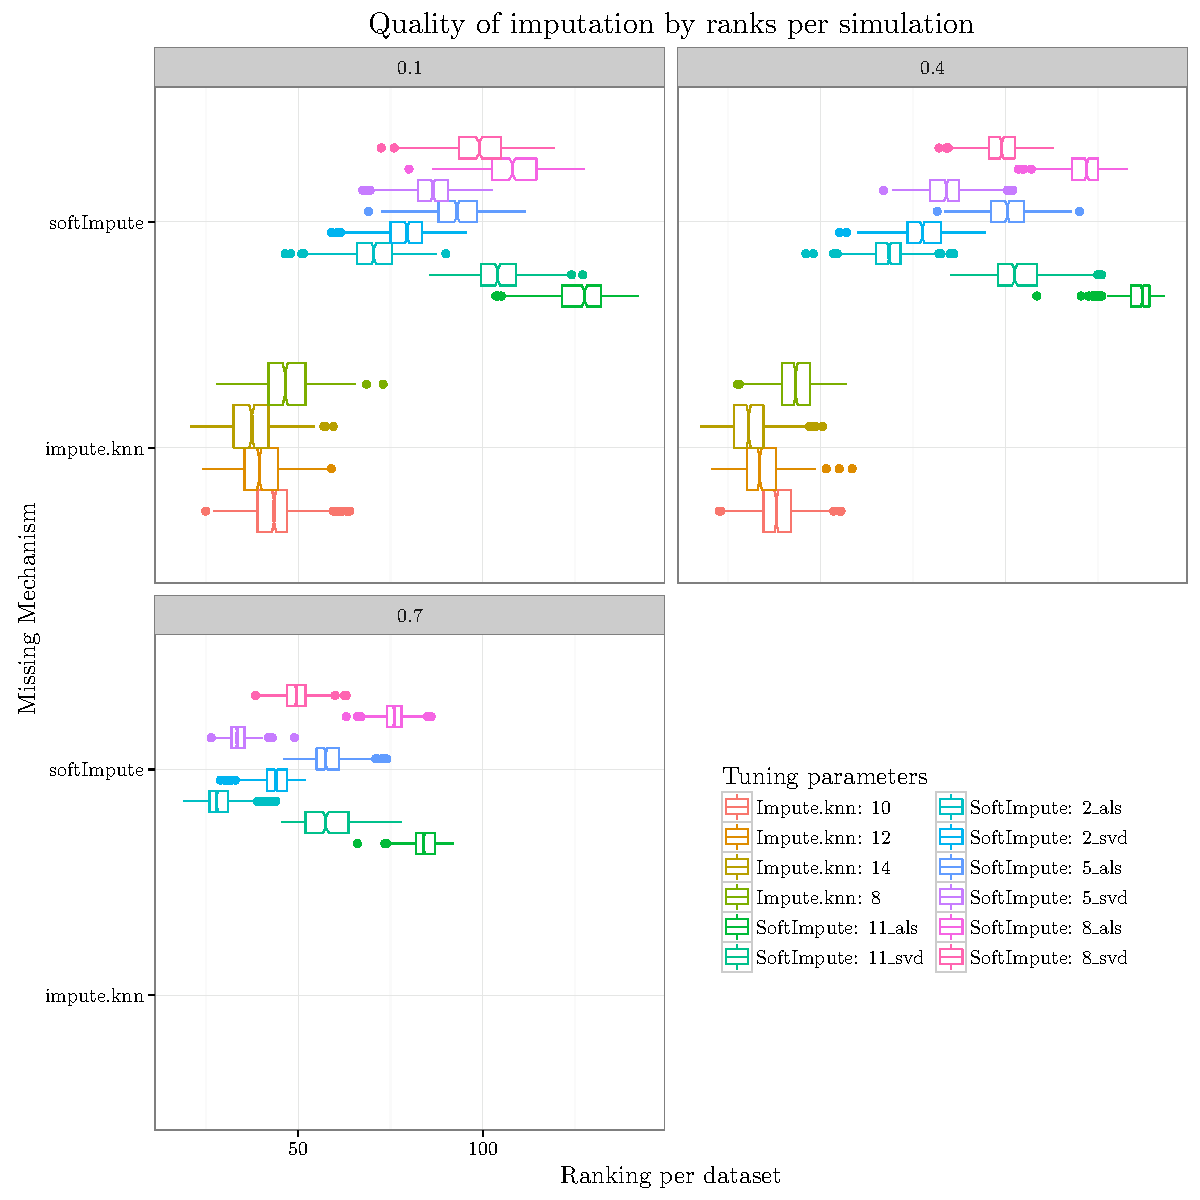
\includegraphics[width=\textwidth]{tuning_ranking_soft_impute_plot}
  \caption{Relative ranking of imputation quality of the tuning parameters of
    softImpute and impute.knn. For impute.knn, the number of neighbors is the
    tuning parameters, whereas for softimpute, it is the maximum rank and estimation
    method of the output matrix.}
  \label{fig:tuning:param:softimpute:imputeknn}
\end{figure}

\paragraph{Tuning parameters}
For the packages \texttt{softImpute} and \texttt{impute}, some defaults
parameters for the imputation methods are provided. Figure
\ref{fig:tuning:param:softimpute:imputeknn} displays how the quality of the
imputation evolves with the parameters. The \texttt{impute.knn} function, the
quality of the inference grows with the number of neighbors. The
\texttt{softImpute} function unexpectedly offers good default parameters, even
if some restrain should be kept when the missing rate is high.

\section{Results}

Figure \ref{fig:ranking:imputations} summarize the results under the
\textsc{mcar} missing mechanism. \texttt{softImpute} and \texttt{MICE} were the
only package able to cope with a quite high missing rate ($p \geq
0.7$). \texttt{impute.knn} from the \texttt{impute} package, when it works, is
almost always the method with the best score, as defined in Equation
\eqref{eq:score:imputation}. \texttt{MICE} offers a good balance between speed,
robustness and quality of imputations, but the methods depends on the linear
dependency of the columns of the data matrix. Although \texttt{softImpute} can
cope with almost any type of data matrix, its inferences are sub-par with the
other methods. Some further analysis might be needed to confirm this
results. \texttt{Amelia} is the package which is the least able to cope with a
random impute matrix: routines failed without exception with any missing rate
above $p > 0.3$. The \texttt{Amelia} and \texttt{mi} packages use by default
parallel back-ends to perform their computations. However, they are the slowest
methods in terms of elapsed time. This might be overcome by setting the number
of iteration to a lower threshold. Nonetheless, this is not recommended as
convergence is not guaranteed when data input might have dimensions with strong
linear dependency.

Figure \ref{fig:mse:mcar} shows the measure from Equation \eqref{eq:smse} for
missingness rates $p \in \{0.2, 0.5, 0.7\}$. For numerical data, all methods
but \texttt{softImpute} have the same order of errors with K-nearest neighbors
being slightly better than the others. However, the latter method does not
allow for inference of the imputation error.  As Figure \ref{fig:mse:mar}
shows, the previous statements are not impacted by changing the missingness
mechanism to (our implementation of) \textsc{mar}.

\section{Open questions}

Heuristically, the quality of models output normally depends on the amount of
available data. In the missing data framework, precision are needed for this
notion: Is it the number of complete observations, the number of non-missing
values, or a mixture of both?  Interactions between the number of observation
$n$, the number of dimensions $p$ and imputation methods with their optimal
parameters are left unanswered with this work. In order to answer this
question, a multivariate sampling mechanism should be devised and tested.

Moreover, are there any reasonable solutions which can be applied to overcome
collinearity? One could cluster the similar dimension and then pick one randomly
to create an imputed value. Nevertheless, such solutions were not yet
implemented.

Additionally, this small simulation study has been applied to certain data set
and it should be interesting to repeat the experience with other real data.

Finally, the concern of this work has been to apply imputation methods to
retrieve potential candidate values for inference, it would have been
interesting to verify the quality of inferences performed with the imputed data
set, for example multiple imputation against nearest neighbors.


\begin{figure}
  \centering
  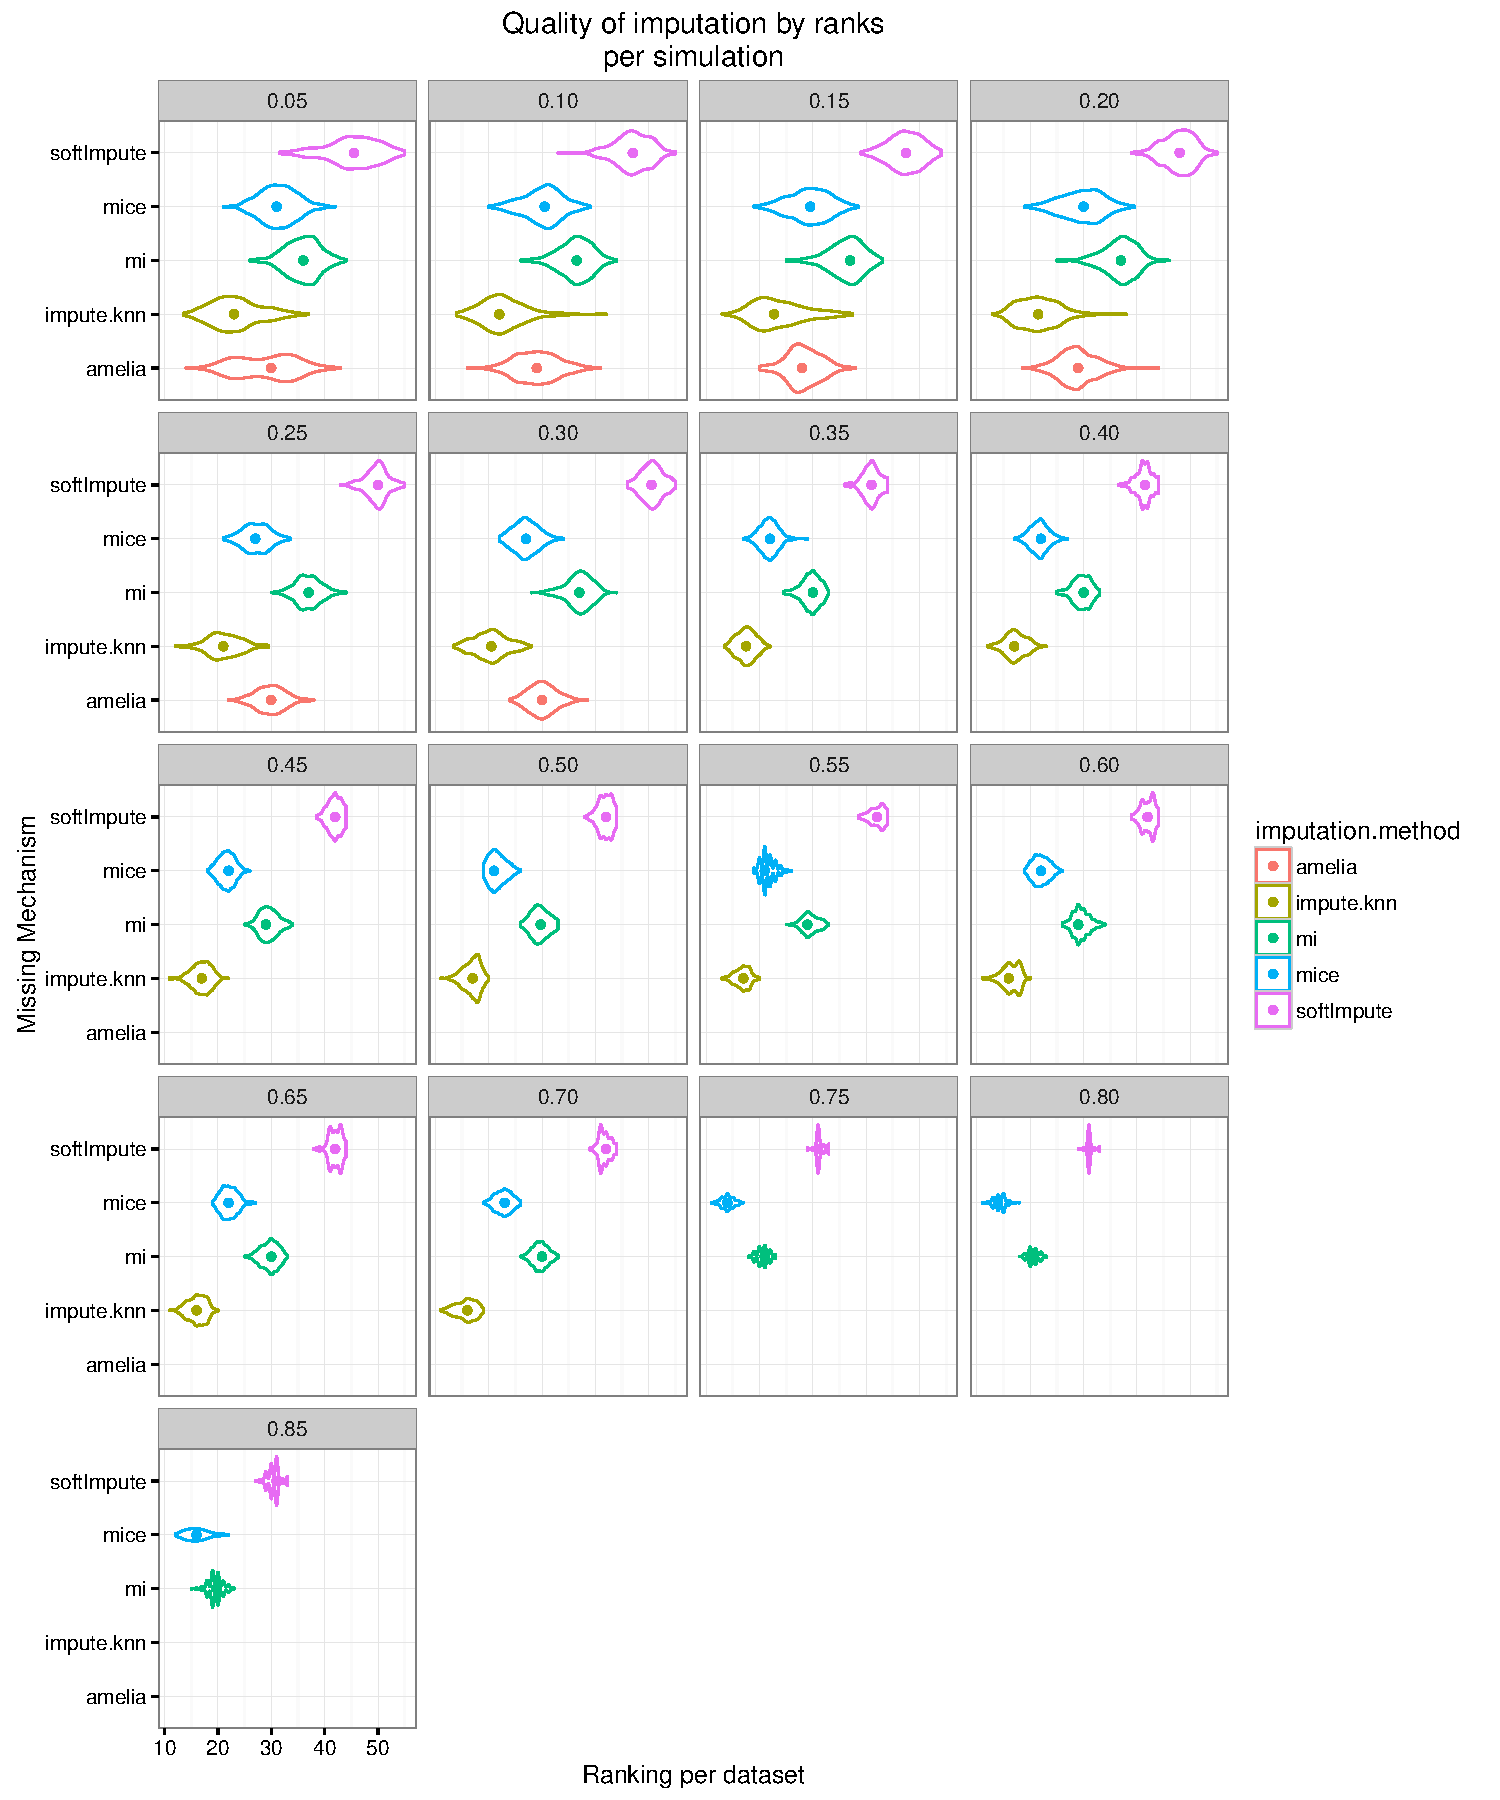
\includegraphics[width=\textwidth]{partial_ranking_plot}
  \caption{Rankings of imputation methods on the FLAS data set grouped by
    missing rate, under the MCAR mechanism with missing rate. Labels in the
    boxes provide the missing rate.}
  \label{fig:ranking:imputations}
\end{figure}


\begin{figure}
  \centering
  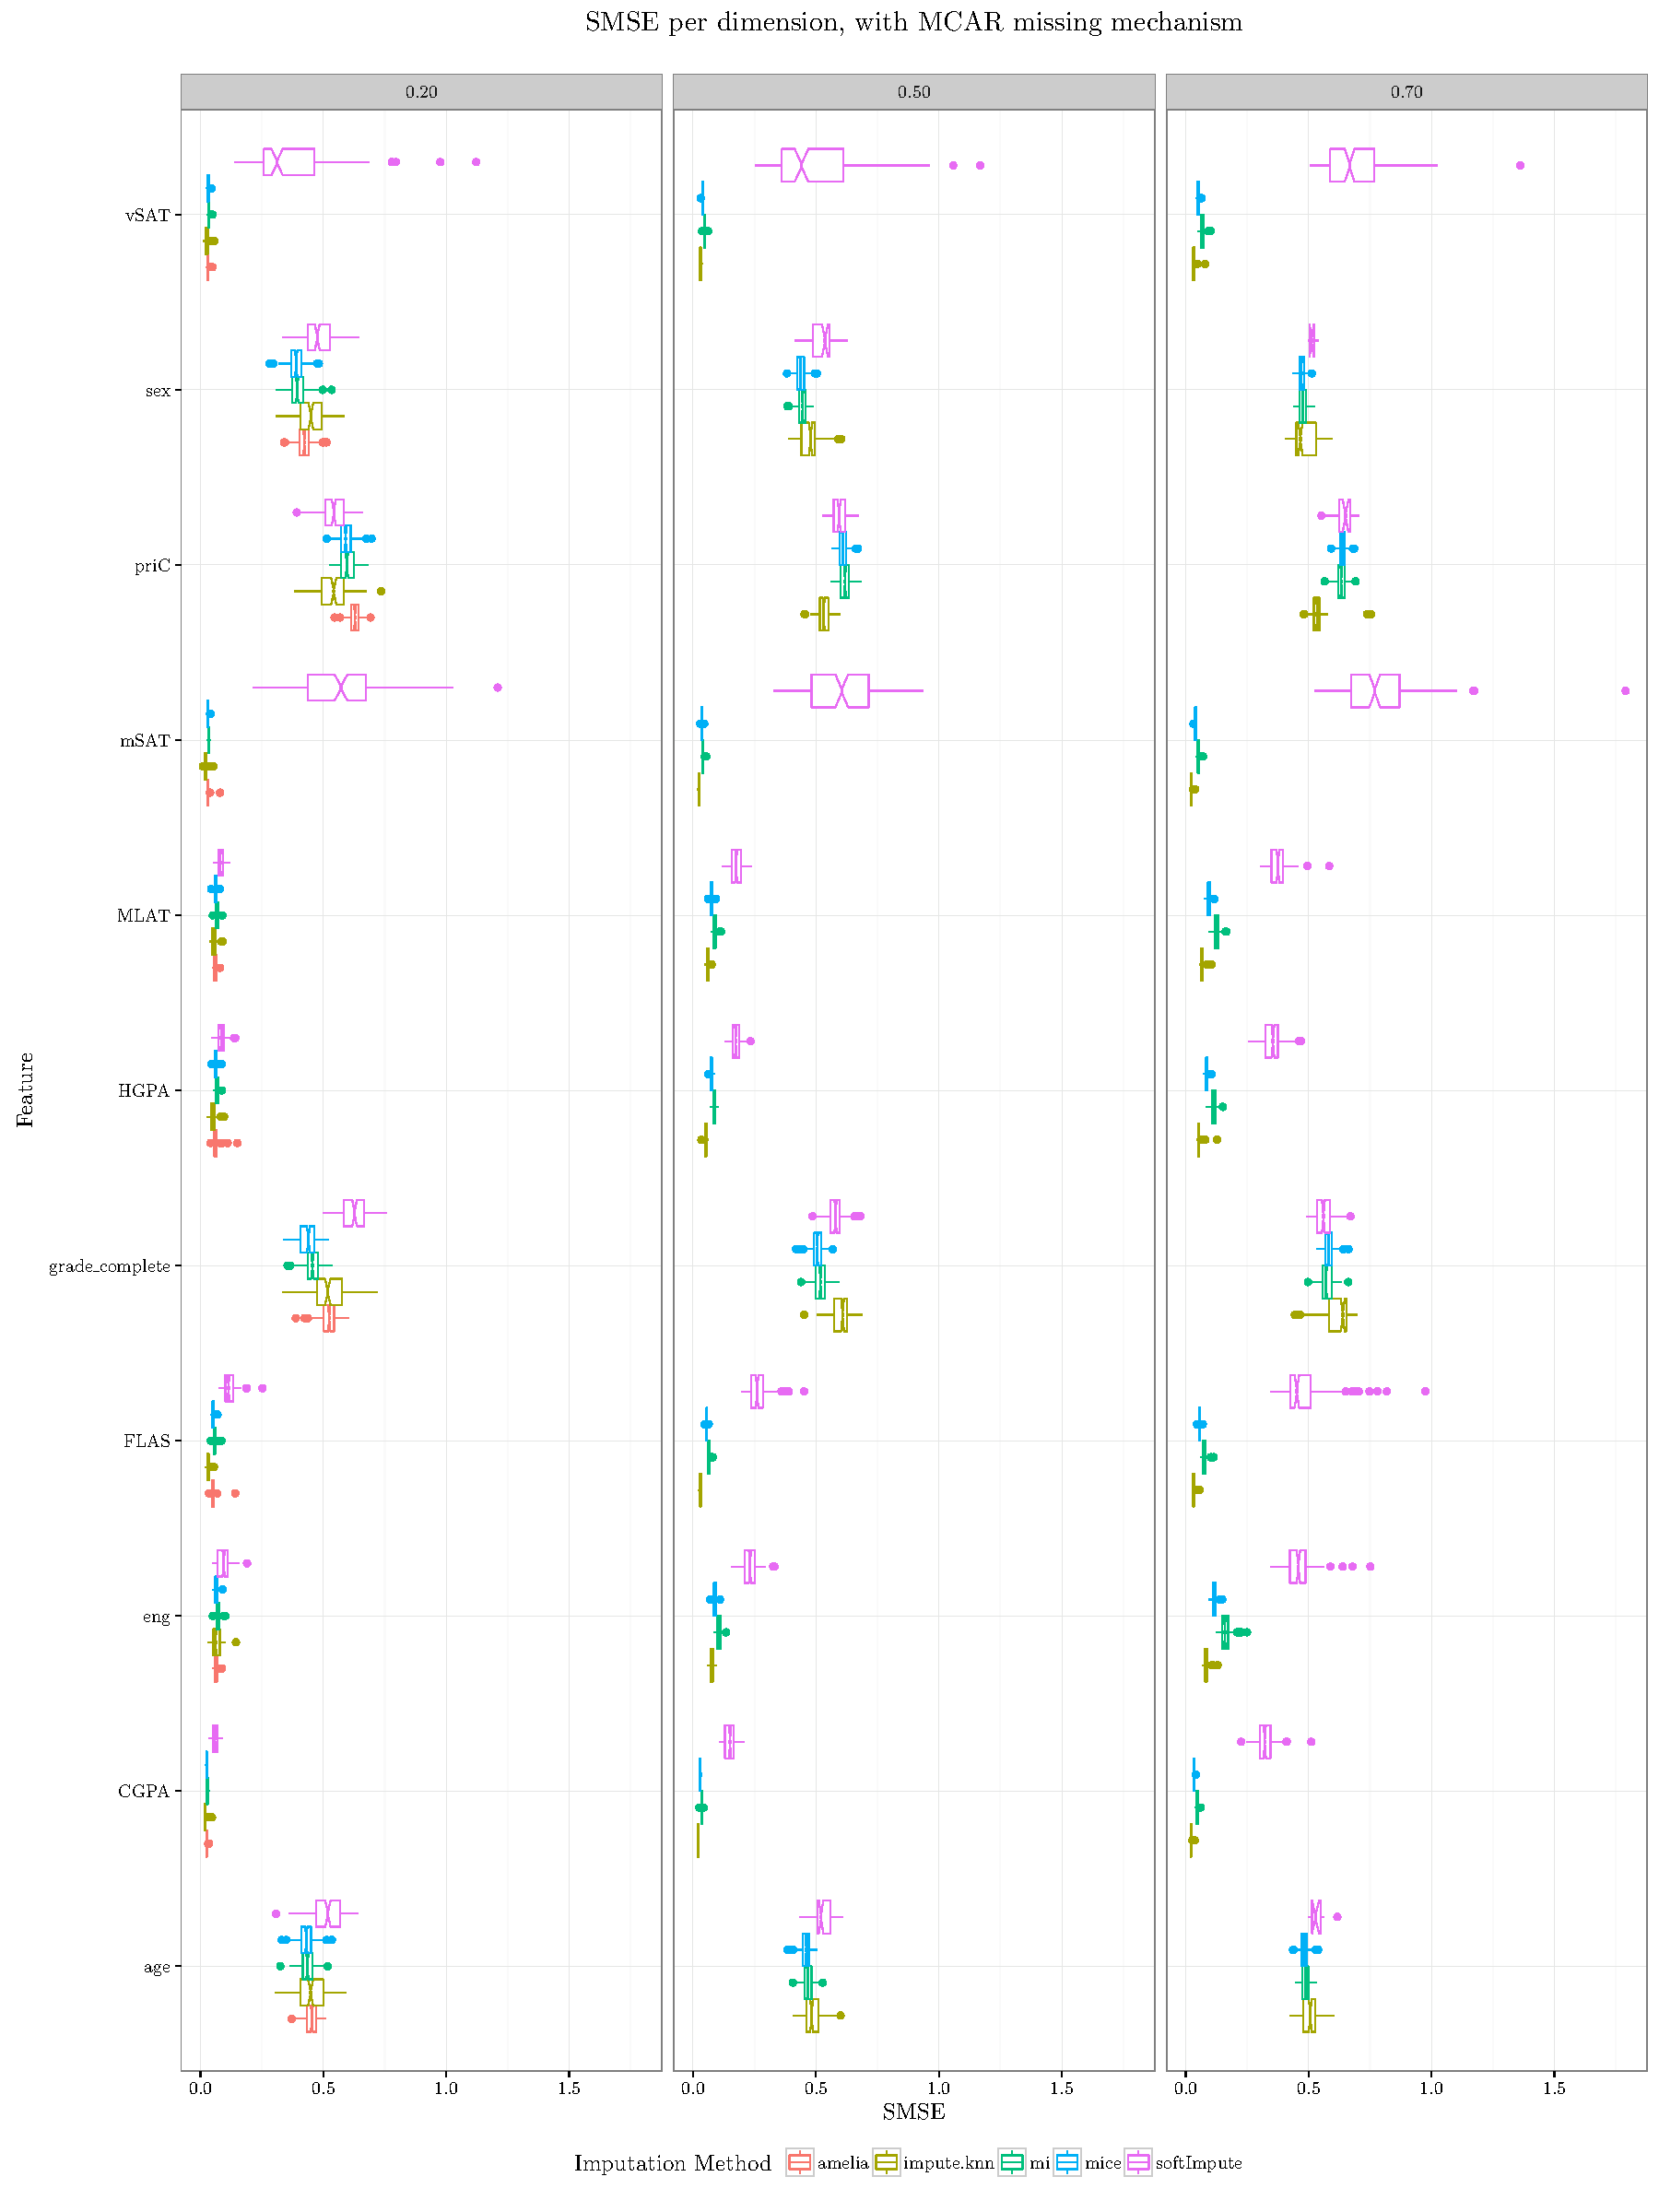
\includegraphics[width=\textwidth]{partial_mcar_measures_prob_selection}
  \caption{SMSE for selected missingness rate with MCAR
    against imputation methods.}
  \label{fig:mse:mcar}
\end{figure}


\begin{figure}
  \centering
  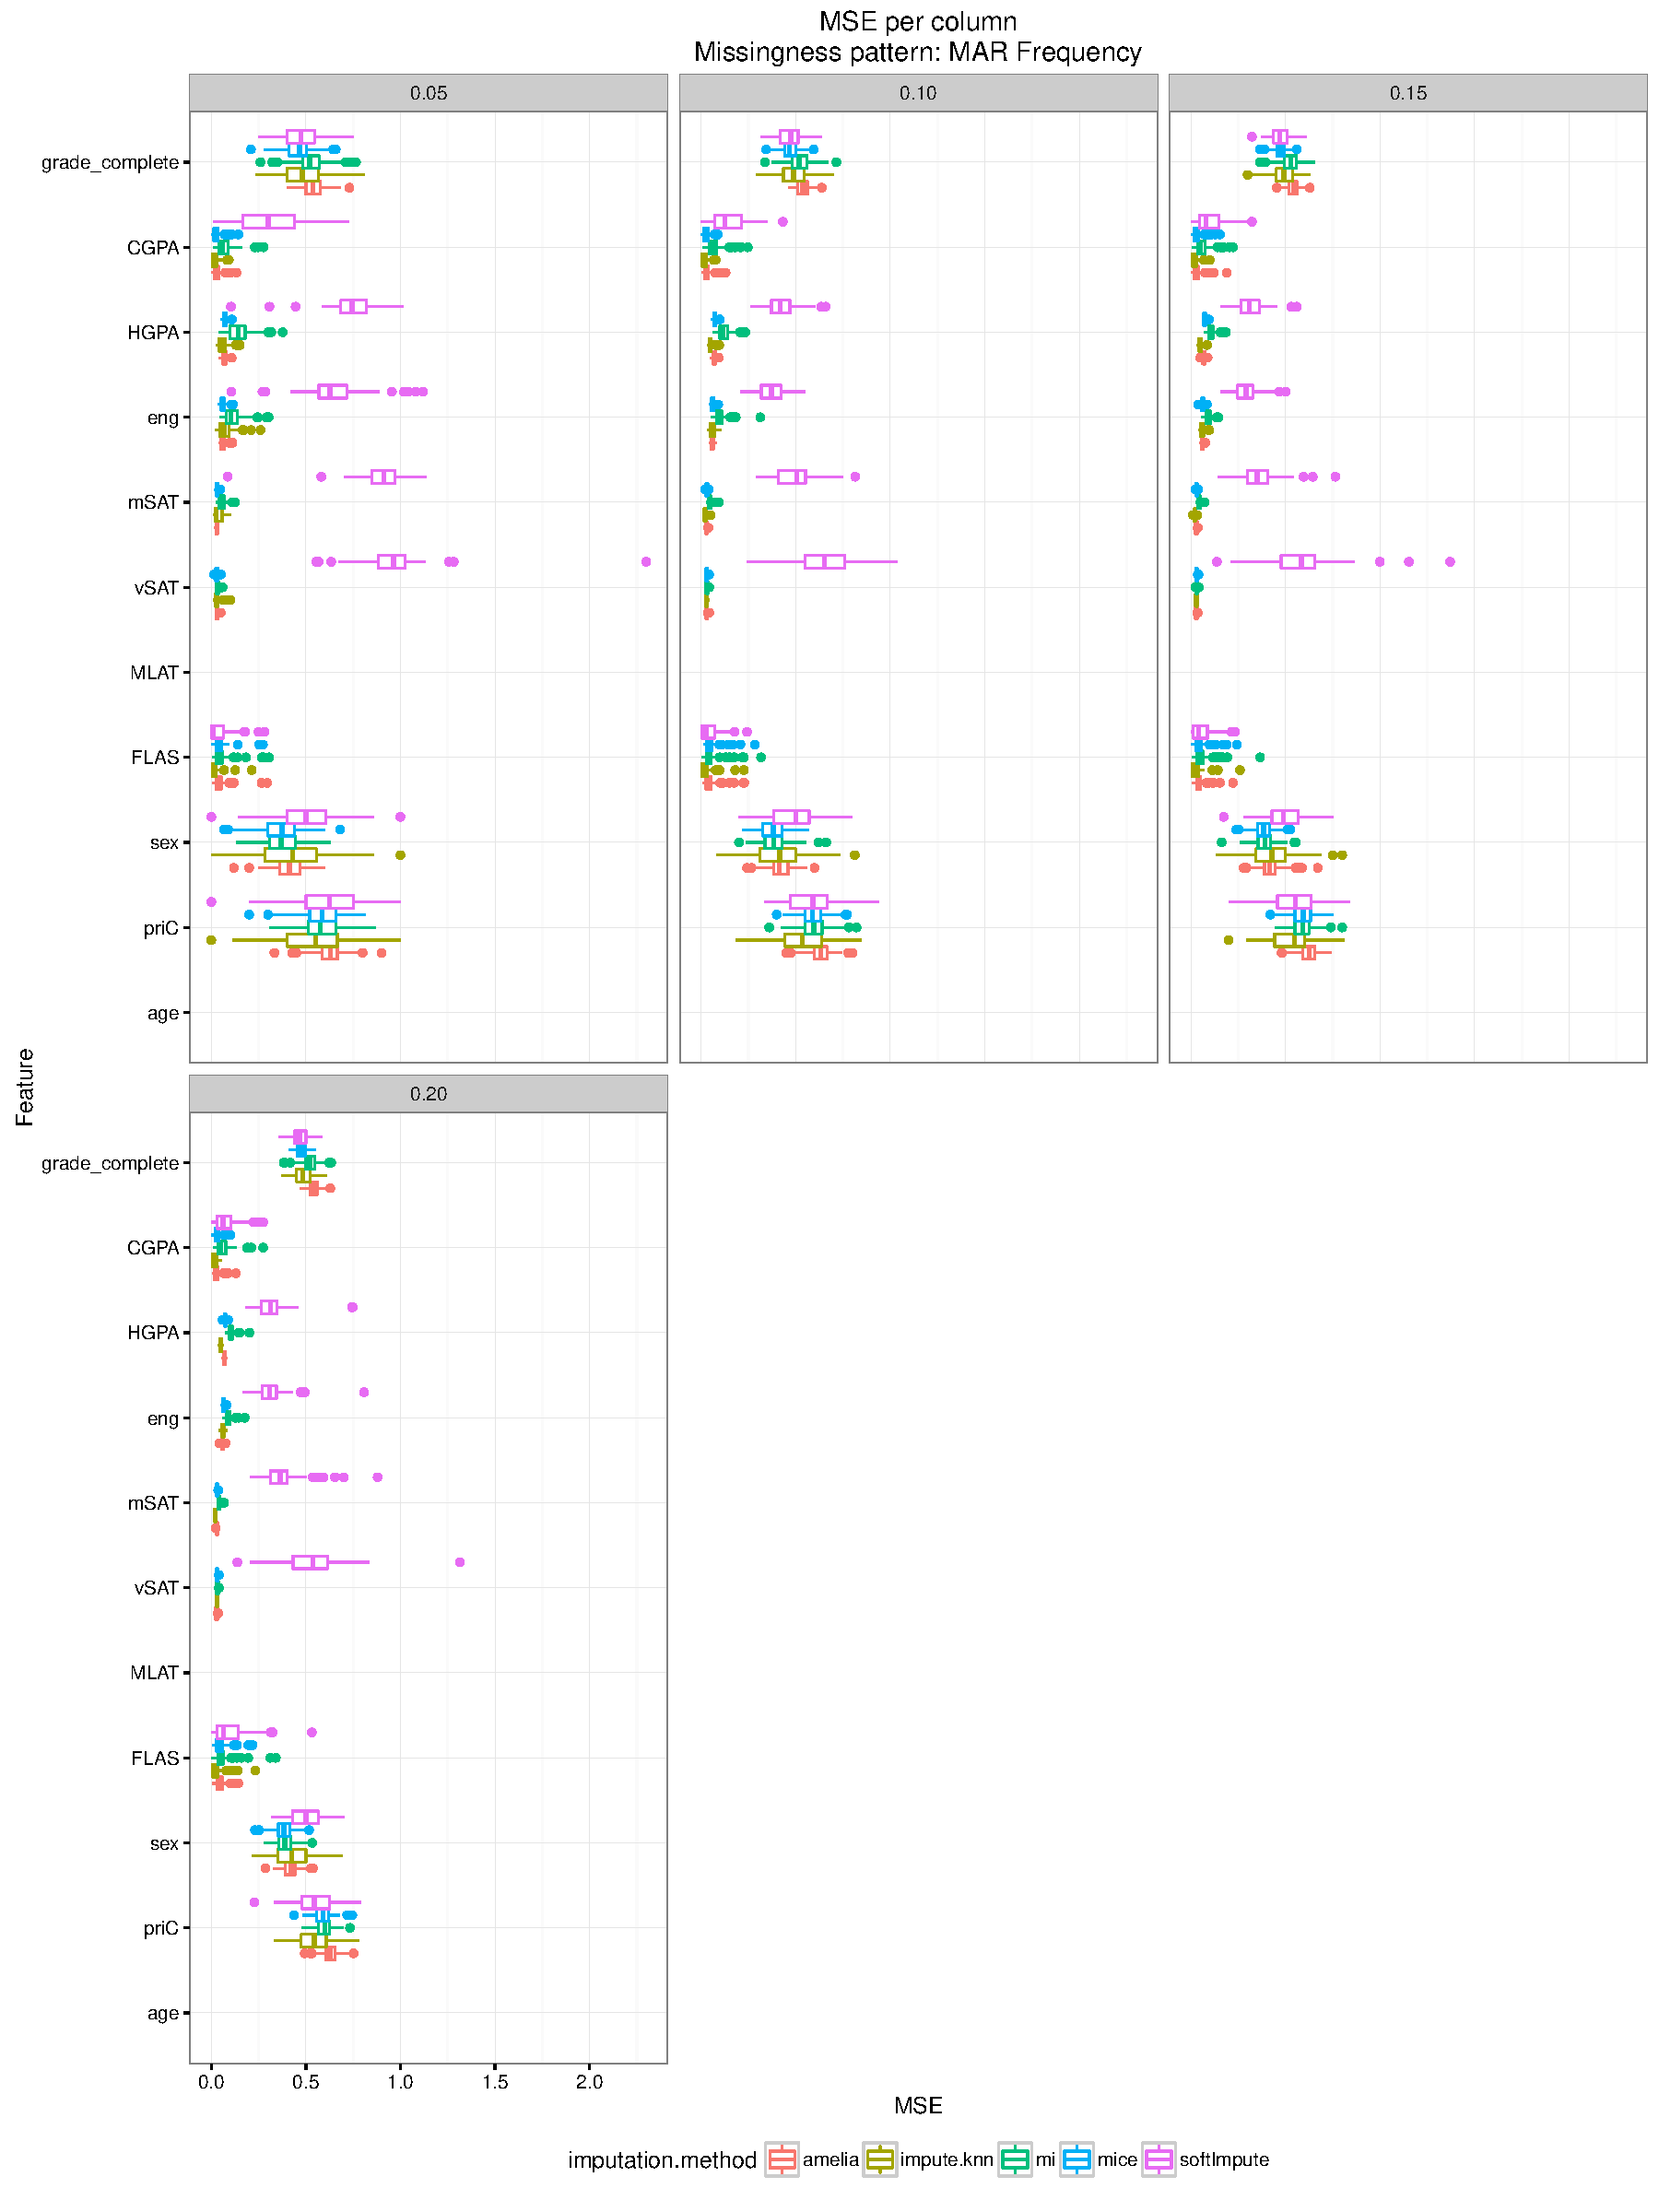
\includegraphics[width=\textwidth]{partial_marfrequency_measures}
  \caption{SMSE of imputation methods on the FLAS data set grouped by missing
    rate, under the MAR mechanism. Labels in the boxes provide the missing
    rate.}
  \label{fig:mse:mar}
\end{figure}



%%% Local Variables: ***
%%% mode:latex ***
%%% TeX-master: "semester_paper_sfs.tex"  ***
%%% End: ***
%%% reftex-default-bibliography: ("biblio.bib")
 % Empirical results % Description of data set
% \chapter{Summary}
\label{s:Summary}

Summarize the presented work. Why is it useful to the research field or institute?


\section{Future Work}
\label{ss:FutureWork}

Possible ways to extend the work.


%%% Local Variables: 
%%% mode: latex
%%% TeX-master: "MasterThesisSfS"
%%% End: 


%%%%%%%%%%%%%%%%%%%%%%%%%%%%%%%%%%%%%%%%%%%%%%%%%
%%% Bibliography                              %%%
%%%%%%%%%%%%%%%%%%%%%%%%%%%%%%%%%%%%%%%%%%%%%%%%%
\addtocontents{toc}{\vspace{.5\baselineskip}}
\cleardoublepage
\phantomsection
\addcontentsline{toc}{chapter}{\protect\numberline{}{Bibliography}}
\bibliography{biblio.bib}
%% All books from our library (SfS) are already in a BiBTeX file
%% (Assbib). You can use Assbib combined with your personal BiBTeX file:
%% \bibliography{Myreferences,Assbib}. Of course, this will only work on
%% the computers at SfS, unless you copy the Assbib file
%%  --> /u/sfs/bib/Assbib.bib

%%%%%%%%%%%%%%%%%%%%%%%%%%%%%%%%%%%%%%%%%%%%%%%%%
%%% Appendices (if needed)                    %%%
%%%%%%%%%%%%%%%%%%%%%%%%%%%%%%%%%%%%%%%%%%%%%%%%%
% \addtocontents{toc}{\vspace{.5\baselineskip}}
% \appendix
% \chapter{R Implementation Details}
\label{app:complement}

The complete \textsf{R} code to generate the result is stored on
\url{https://github.com/davidpham87/ethz\_missing\_data} where the procedure
are well documented.

\section{Completion of the original FLAS data set}

One of the critical element in the comparison of completion methods is the
complete data set from which the artificial incomplete data set is derived. As
explained, the original FLAS data set contains missing value and the following
steps to complete it are described below.

For each of the \texttt{mice} and \texttt{mi} packages, 20 imputed data set are
created. The selected final observation is then either the arithmetic average
for numerical variables or the mode for factor variables among the 40 imputed
data set and it becomes the baseline for all the comparison.

\lstinputlisting[language=R, style=Rstyle]{../../R/flas_completion.R}

\section{Generation of low-level errors}

If the reader is interested in looking at the output of these script, they are
available on
\url{github.com/davidpham87/ethz_missing_data/tree/master/R/bug_replication}.

\paragraph{Amelia}

\texttt{Amelia}'s implementation seems to have difficulties to handle some
structures of data matrix with missing values. The following code snippet shows
how to reproduce this errors.

\lstinputlisting[language=R, style=Rstyle]{../../R/bug_replication/bug_amelia.R}

\paragraph{Impute}

The \texttt{impute} package seems to call an underlying \texttt{fortran}
procedure. The call can throw some segmentation fault errors depending on
the nature of some arguments.

\lstinputlisting[language=R, style=Rstyle]{../../R/bug_replication/bug_impute_knn.R}

%%% Local Variables:
%%% mode: latex
%%% TeX-master: "semester_paper_sfs"
%%% End:

% \chapter{Yet another appendix....}

\section{Description}
\begin{description}
\item[Something] details.
\item[Something else] other definition.
\end{description}

\section{Tables}
Refer to Table~\ref{tab:example} to see a left justified table with caption
on top.

\begin{table}[ht]
\centering
\caption[Test results]{\label{tab:example}Results.}
\begin{tabular}{ll}
\hline
\textbf{Student} & \textbf{Grade}\\
\hline
Marie  & $6$\\
Alain  & $5.5$\\
Josette  & $4.5$\\
Pierre  & $5$\\
\hline
\end{tabular}
\end{table}

%%% Local Variables: 
%%% mode: latex
%%% TeX-master: "MasterThesisSfS"
%%% End: 



% %% Epilogue (optional)
% \addtocontents{toc}{\vspace{.5\baselineskip}}
% \cleardoublepage
% \phantomsection
% \addcontentsline{toc}{chapter}{\protect\numberline{}{Epilogue}}
% \markboth{Epilogue}{Epilogue}
% \chapter*{Epilogue}
\label{s:Epilogue}

A few final words.



%%% Local Variables: 
%%% mode: latex
%%% TeX-master: "MasterThesisSfS"
%%% End: 


%%%%%%%%%%%%%%%%%%%%%%%%%%%%%%%%%%%%%%%%%%%%%%%%%%
%%% Declaration of originality (Do not remove!)%%%
%%%%%%%%%%%%%%%%%%%%%%%%%%%%%%%%%%%%%%%%%%%%%%%%%%
%% Instructions:
%% -------------
%% fill in the empty document confirmation-originality.pdf electronically
%% print it out and sign it
%% scan it in again and save the scan in this directory with name
%% confirmation-originality-scan.pdf
%%
%% General info on plagiarism:
%% https://www.ethz.ch/students/en/studies/performance-assessments/plagiarism.html
\cleardoublepage
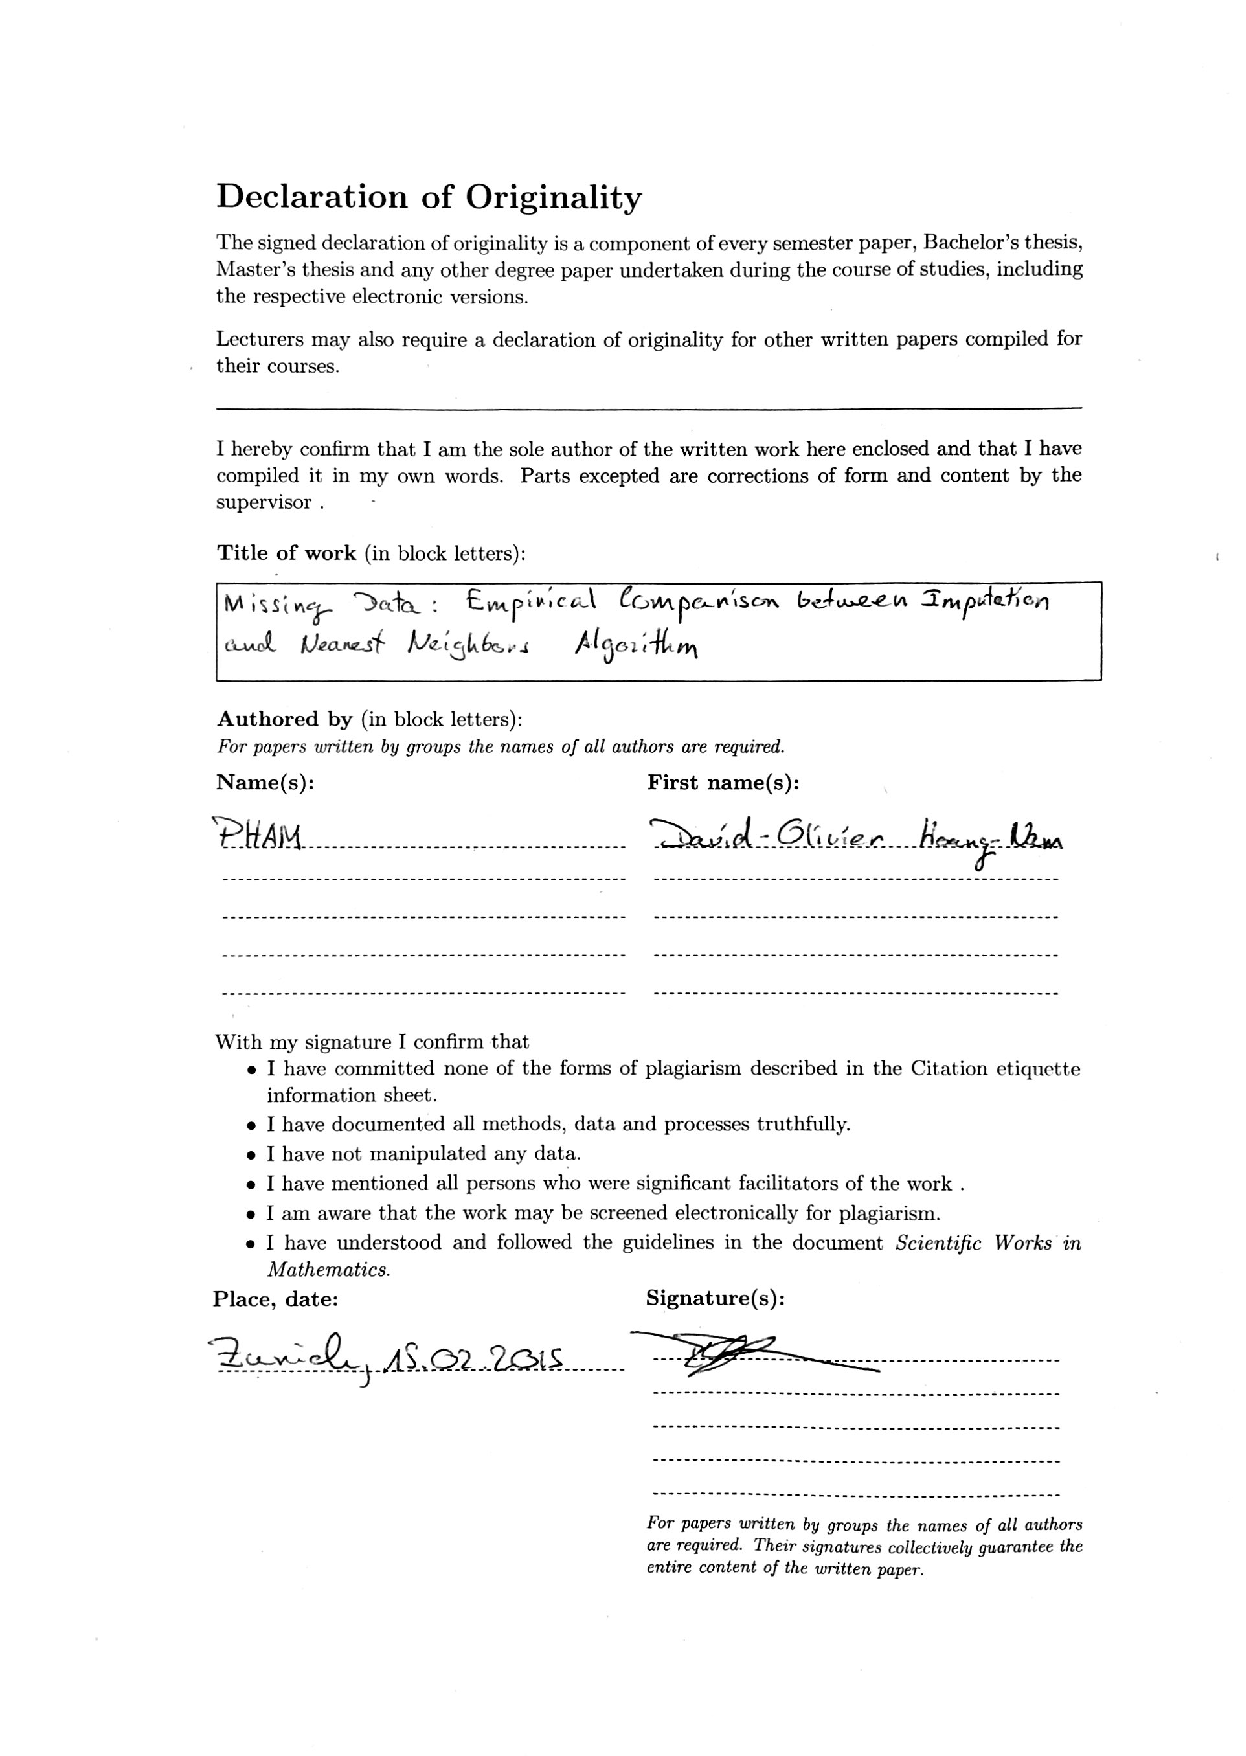
\includepdf[pages={-}, frame=true,scale=1]{confirmation-originality-scan.pdf}
\end{document}
